\documentclass[article]{aaltoseries}
\usepackage[utf8]{inputenc}
\usepackage{url}


\begin{document}
 
%=========================================================

\title{Digital Twins for Industrial Edge 4.0: Concepts and Tools}

\author{Adika Bintang Sulaeman% Your first and last name: do _not_ add your student number
\\\textnormal{\texttt{adika.sulaeman@aalto.fi}}} % Your Aalto e-mail address

\affiliation{\textbf{Tutor}: Prof. Hong-Linh Truong} % First and last name of your tutor

\maketitle

%==========================================================

\begin{abstract}
  Industry 4.0 is expected to be the next big phase in industry. Digital Twins (DT), defined as digital representations of physical objects such as machines, have an important role in Industry 4.0. This seminar paper discusses an overview of DT technology, key technologies to implement DT, DT frameworks, and supporting technologies to realize the DT framework. From the literature study conducted, the existing works from previous research can support the DT framework to implement DT systems.
  
\vspace{3mm}
\noindent KEYWORDS: Digital Twin, Industrial Internet of Things, Industry 4.0

\end{abstract}


%============================================================


\section{Introduction}

Industry 4.0 is the next big phase in industry. With Industry 4.0, it is possible to gather real-time data from the machines that run in industry and process the data into something meaningful and useful. Industry 4.0 mainly consists of three supporting technologies: IoT, Cyber-Physical Systems (CPS), and Smart Factories \cite{hermann2016design}. The combination of these technologies builds interconnected devices forming Digital Twins (DT).

A DT models a physical object by creating a digital representation using real-time data \cite{Cheatshe3:online}. The data is gathered throughout its life-cycle and used as the source to monitor, learn from, and enhance decision making. A DT enables engineers to monitor and understand how the machines behave once it is released and run by users. Furthermore, engineers can analyze the data and predict the future performance of the machines.

There are some use cases of DT for Industry 4.0. Consider a Printed Circuit Board (PCB) printer for electronic manufacturers. The PCB printer must be very precise, because the smallest error by the laser cutter may lead to PCB flaws. A DT enables engineers and technicians to monitor and analyze the data to predict the time when the spare parts wear out. Another example would be monitoring the jet engine of airplanes. By analyzing data gathered in real-time, engineers and technicians may predict failures in jet systems, which will lead to the reduction of airplane incidents. Furthermore, DT may give feedback to the engineers who design the machine to help them realize an agile development system.

The main value that the DT delivers is an understanding of product performance \cite{Cheatshe3:online}. By understanding performance, manufacturers may detect and understand faults better, create an effective maintenance schedule, troubleshoot machines remotely, and decide appropriate add-on services.

The DT has some challenges in its development and implementation. In \cite{bienhaus2017patterns}, the author has stated a number of challenges such as data consistency between the real physical assets and the digital representation, as well as connectivity and security concerns of cloud computing for DT. Software architectural aspects such as internal structure, APIs, integration, and runtime environment are also critical challenges for DT \cite{malakuti2018architectural}.

\subsection{Scope and Goals}
\label{sec:emphasis}
This paper aims to review the concept of DT for manufacturing in Industry 4.0 as well as technologies to build the DT system. This seminar paper is intended as a review paper for DT developers to build DT system.

\subsection{Structure}
\label{sec:em}
The rest of this paper is organized as follows. Section 2 discusses the key technologies for DT. Section 3 discusses the existing DT framework approaches and supporting technologies to build the DT framework. Section 4 concludes this review paper.
 

%============================================================



%============================================================

\section{Key Technologies for Digital Twins}
The entity of DT elements can be modeled as a five-dimension DT \cite{Tao2019}. The five-dimension model consists of Physical Entity (PE), Virtual Entity (VE), Services (SS), DT Data (DD) and Connection (CN). Each of these components requires technologies to implement in order to form DT.

\subsection{Physical Entity (PE)}
PE is the real physical entity in the physical space. It contains the real machines with their sensors and actuators. The sensors attached to the PE capture the data from PE during its operation.

To enable PE as DT elements, some technologies are needed. First of all, an embedded system is needed on every PE. The computing capabilities embedded in PE is used for reading the data from the sensors and format the data before sent to other DT elements. Secondly, the Wireless Sensor Network (WSN) is the backbone of the communication of the sensors data. Other relevant technologies such as distributed sensor layout optimization to reduce redundancy of sensor data, soft sensor to calculate PE's partial parameters, and RFID to track and identify the PE have an important role in DT.

\subsection{Virtual Entity (VE)}
VE consists of a set of models representing the PE. Modeling techniques such as three-dimension solid modeling, physics modeling, behavior modeling, and rule modeling are needed to create useful modeling of the PE. To keep PE and VE model consistent, model consistency analysis, verification, validation and accreditation must be implemented. These techniques may form solid representation models of the PE. The models can be combined with Virtual Reality (VR) and Augmented Reality (AR) to create a similar environment to the physical space.

\subsection{Services (Ss)}
The software services of the DT is intended to be consumed by PE and VE. The services used by PE includes monitoring service, state prediction service, and energy consumption optimization service. VE uses the construction service, calibration service and test service for models.

There are some aspects that need to consider to develop services for modeling DT. Resource management for collecting, classifying, and organizing resources in the DT is an important aspect for the services. The services must also be able to transform resources into software services through digital services. Fault-tolerant management is also important to mitigate failures caused by networks, services, sudden high demands of applications. Human-machine interface is also important to enable interaction between users and services.

\subsection{DT Data (DD)}
DD have data from physical and virtual parts. Therefore, there are a massive amount of heterogeneous data. Technologies for processing and securing data including data storage, data modeling, data transformation, data cleaning, data analysis, data mining, data integrity check and data security are required in helping modeling DT data.

\subsection{Connection (CN)}
CN connects different elements of DT. It enables PE, VE, Ss, and DD to communicate with each other. Key technologies of CN includes communication protocol analysis, communication protocol/interface conversion, wireless communication, Application Programming Interface (API) design, as well as communication standard and specification.

\section{Implementing Digital Twin Systems}
Several researchers have proposed frameworks for implementing DT. This section discusses and analyzes the approaches proposed by researchers.

\subsection{DT Frameworks}
Yu Zheng et. al. proposed an application framework of DT to realize full-physical system mapping, life-cycle dynamic modeling and the whole process real-time optimization \cite{zheng2019application}. This application framework consists of three elements, i.e., physical space, virtual space and information-processing layer. Fig.~\ref{fig:app_framwork_zheng} shows the application framework and the interaction among the physical space, virtual space and information-processing layer.

\begin{figure}[t!]
	\begin{center}
		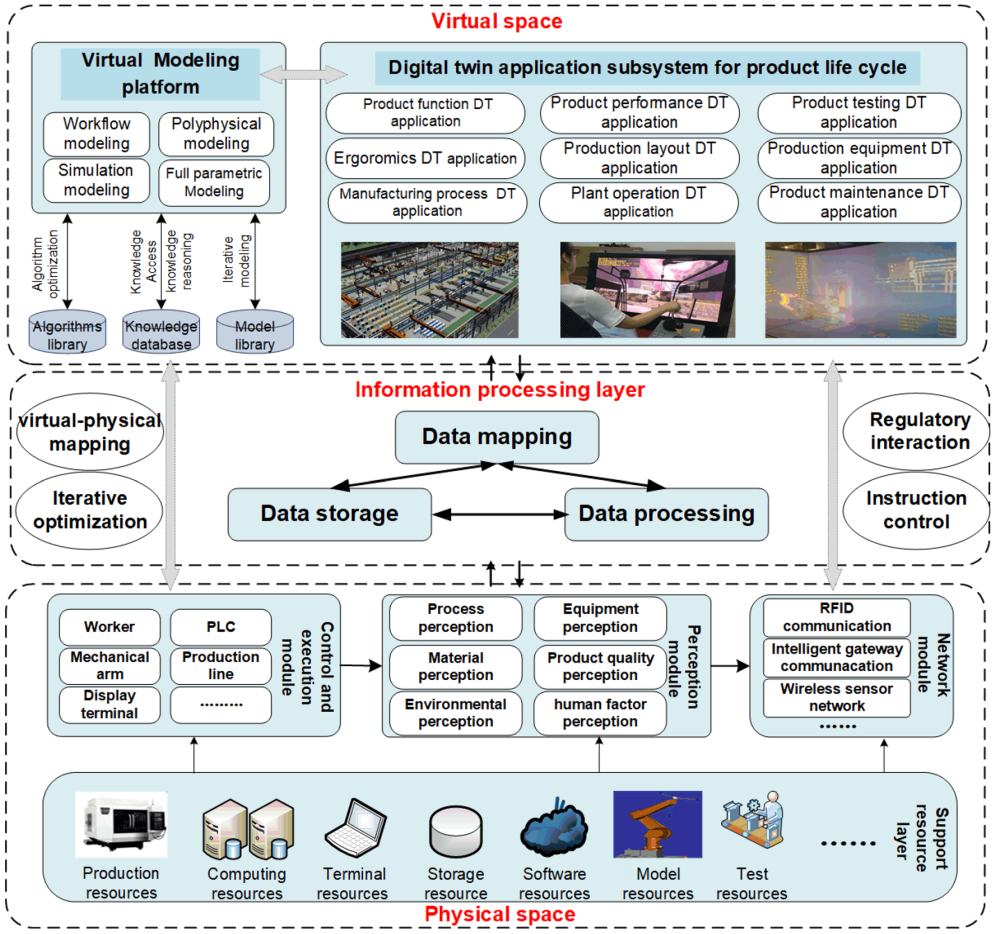
\includegraphics[width=1\textwidth]{figures/app_framework_yu_zheng_et_al}
		\caption{Application Framework for DT \cite{zheng2019application}}
		\label{fig:app_framwork_zheng}
	\end{center}
\end{figure}

The physical space of the framework consists of human workers, machines, materials, rules, and the environment. These complex and diverse objects are connected by IoT or WSN technologies. In a manufacturing workshop, for example, sensors and communication equipment collect and deliver data from the physical space such as equipment attributes, status, process, fault and error. Mechanisms and techniques for mapping data to devices are needed to infer the interaction between the physical and digital space.

The information processing layer connects the physical space to virtual space. In addition, it provides a bidirectional mapping between physical and virtual space. This layer consists of data storage, data processing, and data mapping modules. Data storage module stores all the data from both physical and virtual space. Data processing module deals with data acquisition, data processing, data analysis, and data fusion. Data mapping utilizes data from storage and processing module to map the operation of physical to virtual space and vice versa.

The virtual space consists of the Virtual Environment Platform (VMP) and DT application subsystem for product lifecycle management. The VMP models 3D virtual model as well as provides an operating environment for DT related algorithms. VMP provides virtual models by obtaining data from the database. The data generated from the virtual space is stored as historical data in the database. The combination of historical and real-time data drive the DT application subsystems work synchronously.

Zhuang et. al. proposed DT-based smart production management and control framework for product assembly shop-floor \cite{Zhuang2018}. The framework consists of four techniques in which each of them need a sub-framework to operate: (1) real-time acquisition, organization, management of the physical space, (2) construction of the virtual space of the shop-floor, (3) DT and big-data driven prediction and (4) production management and control service of the assembly shop-floor. Fig.~\ref{fig:zhuang_framework} shows the framework of DT-based production management and control, with satellite assembly shop-floor as the case study.

\begin{figure}[t!]
	\begin{center}
		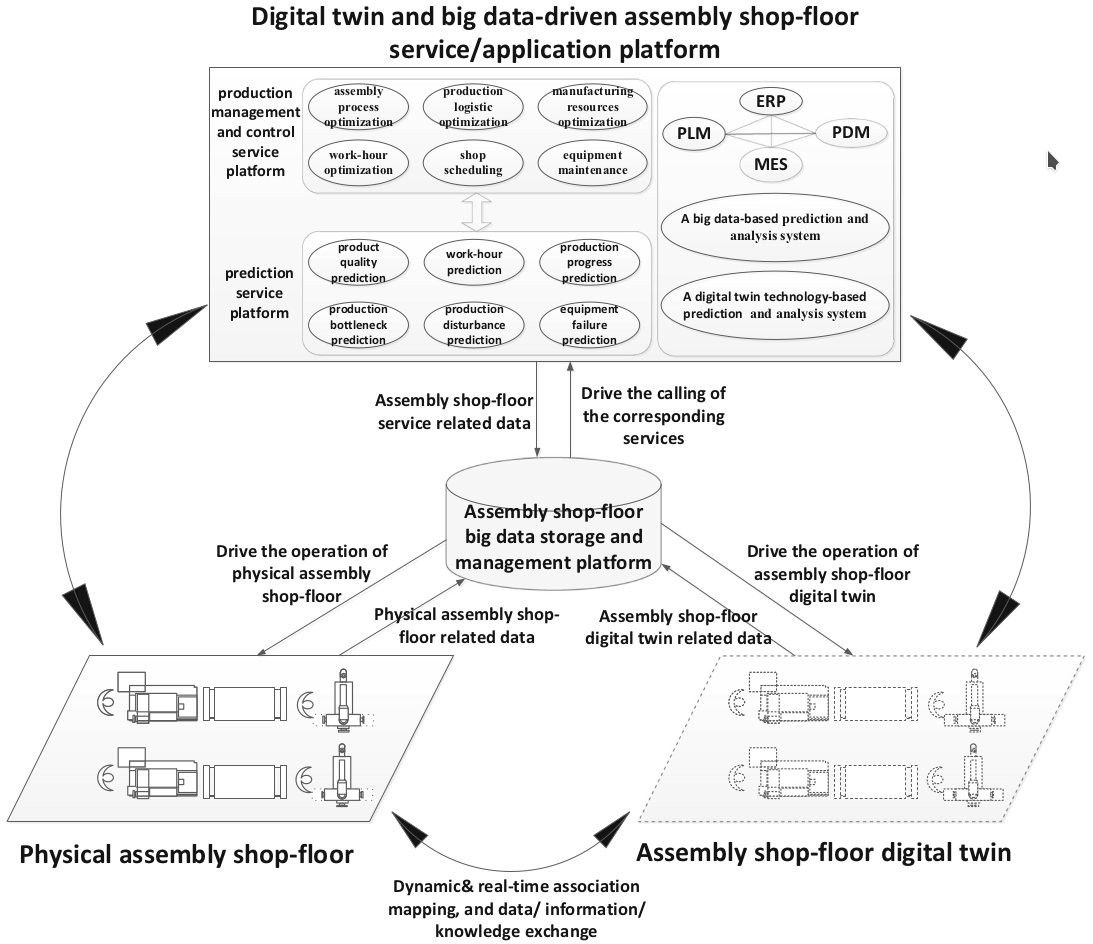
\includegraphics[width=1\textwidth]{figures/zhuang_dt_framework}
		\caption{Framework of DT-based production management and control for satellite assembly shop-floor \cite{Zhuang2018}}
		\label{fig:zhuang_framework}
	\end{center}
\end{figure}

The framework for real-time acquisition, organization and management of physical shop-floor is realized by IoT, workflow, and DT technologies. The smart access to manufacturing resources in the physical space is realized by sensor technologies equipped in the devices. These sensors obtain data to achieve a real-time perception of what happens in the physical space. The data collected from the physical space are categorized into three categories, i.e., the real-time perception, production process, production activity plan. The data organization and management of shop-floor rely on the product Bill of Materials (BOM) which comes from the product design, process planning, and product assembly stage.

The construction of the virtual space is built on three levels, i.e., element, behavior and rule level. The element level models the geometric and physical models using 3D geometric tools such as Pro/E, SolidWorks, CATIA and AutoCAD. The behavior level represents the behavior of the equipment's operations, materials' transportation and personnel's actions using tools such as FlexSim and Unity3D. The rule level consists of rules that govern the association among elements and operation which ensure the match between physical space to virtual space.

The prediction framework relies on big data and DT technologies. The big data framework uses historical data to create a theoretical prediction. The DT uses real-time data to create a simulation which is analyzed by the personnel. The prediction result from both DT and big data is combined to achieve a more accurate prediction.

The production management and control service make real-time decision-making based on the data collected. Furthermore, it also simulates the scheme in the shop-floor. The result of the simulation is used to evaluate the effectiveness of the scheme that is implemented on the shop-floor.

Both frameworks proposed by Zhuang et. al. and Yu Zheng et. al. provide guidelines for implementing DT in manufacturing. The combination of both frameworks may provide a DT system which provides predictive maintenance and product life-cycle management from the developers' perspective. However, there are some works that need to investigate in order to fully implement DT. Further research on the elements of the framework such as the computation models or software architecture in the virtual space, mapping methods between physical and virtual space, methods for data fusion and data processing are needed.

\subsection{Supporting Technologies for DT Frameworks}
In order to implement the DT framework, supporting technologies in IoT, cloud computing, big data and software architecture are needed.

The DT framework starts with collecting and aggregating data from the physical space. Manufacturing Execution System (MES) is commonly used for both collecting data and monitor process and operation of the manufacturing process. MES is generally proprietary and expensive. As a result, small manufacturing enterprise may have difficulties in deploying MES in their system.

Coronado et. al. came up with a low-cost MES system based on Android \cite{UrbinaCoronado2018}. This tool captures part and tooling information using an Android-based MES. The data from MES is combined with data from device sensors to represent parts, operators, capital equipment and consumable in shop-floor DT.

The data collecting and aggregating process starts with device sensors data that is sent using the MTConnect protocol. MTConnect Standard is a protocol for data communication from manufacturing equipment. However, not all equipment are MTConnect compatible, and even some of them do not have communication capability to send data through the network.

To gather further data from the shop-floor that is not accessible by the MTConnect, the Android-based MES is used. For example, operators in the shop-floor can use the MES to register the newly created or modified materials as well as the materials' properties. The data is sent to the cloud where the data is combined with the data coming from the MTConnect protocol. In addition, the MES is also an interface for the operators to see the collected and processed data to support the manufacturing process.

The approach proposed by Coronado et. al. makes the MES integration with the DT more feasible to small enterprises due to the pervasiveness and the low-cost of Android system. However, a concrete design of the software middleware in the cloud is not discussed well.   

A software middleware sits between physical and virtual space to process data from physical space to virtual space and vice versa. Ciavotta et. al. proposed a microservice-based middleware to process data from the CPS which yields output data for DT environment, named MAYA Support Infrastructure (MSI) \cite{ciavotta2017microservice}. It is part of the MAYA Platform; a DT platform consisting of a communication layer, middleware, and simulation framework. The middleware manages the life-cycle of the DT for simulation and synchronizes CPS-to-DT. Fig.~\ref{fig:maya_platform} shows the service diagram of the MSI as well as how it resides in the MAYA platform.

\begin{figure}[t!]
	\begin{center}
		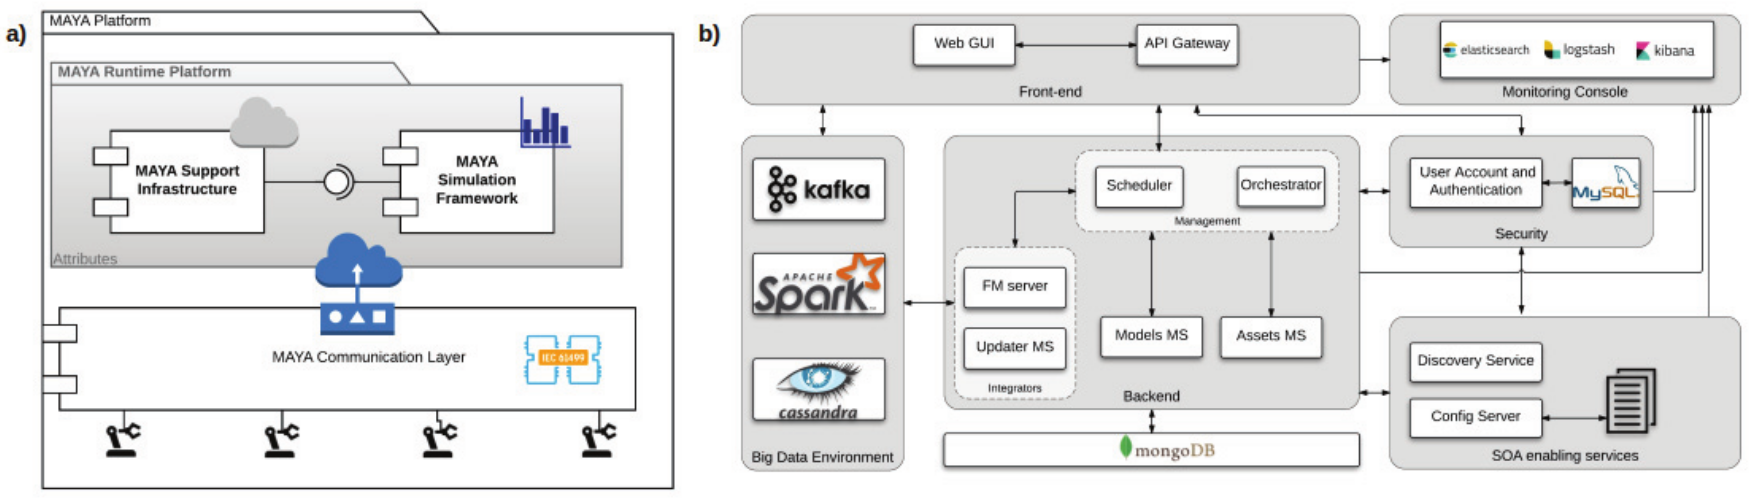
\includegraphics[width=1\textwidth]{figures/maya_platform}
		\caption{a) MAYA platform architecture b) MSI service diagram \cite{ciavotta2017microservice}}
		\label{fig:maya_platform}
	\end{center}
\end{figure}

The middleware is a microservice-based service which consists of five services. The first service is the front-end service which is the interface to the MSI in the form of API gateway and web-based UI. The security service enforces the authentication and authorization using OAuth2. The SOA enabling service has two elements, i.e., the service registry and configuration server. The service registry provides REST endpoint service discovery using Netflix Eureka, and the configuration server stores the configuration properties of the microservice system. Monitoring console service provides system monitoring using Elasticsearch, Logstash, and Kibana (ELK). Finally, the backend service provides create, read, update and delete to DT resources.

There are some benefits of using microservice-based middleware. The microservice technology is known for its agility, isolation and resilience and elasticity. However, it also increases the complexity of the system at the same time.

The MSI middleware still needs further research in communication protocols as implementing IoT-friendly protocol such as MQTT in the front-end service. The middleware also should support standard data exchange format such as Automation Markup Language (AutomationML). Due to its flexibility of the microservice-based middleware, these components can be implemented without re-deploying the whole system.

The service of accepting AutomationML data format is needed in the middleware. Schroeder et. al. demonstrated how to exchange data between systems in DT using AutomationML \cite{Schroeder2016automationml}. In modeling the physical system, AutomationML data format is used to map the components of the automation system. After the model is defined, other systems will use the model to obtain information. Finally, the consumer of the data such as monitoring applications can retrieve the data using RESTful style.

After the aforementioned technologies have been established within the framework, the system must implement visualization technology to imitate the physical objects as the DT. Schroeder et. al. used Augmented Reality (AR) to visualize the twin of the physical object \cite{schroeder2016visualising}. The main idea of the work is the system use web service to get the data of the physical model and supply the data to the visualization system.

The AR system, which provides visualization to the users, query the data of a physical model to the web service. In this case, the web service may have the same architecture as the aforementioned microservice-based middleware. After getting the data from the web service, the visualization is achieved by creating an AR application based on tools such as Vuforia Engine. This work shows that visualizing DT with AR technology can be achieved by getting data from the middleware and provide the data to the visualization system.

\section{Conclusion}
This seminar paper presents an overview of DT technology, key technologies for DT, and DT framework as well as supporting technologies for the DT framework. It starts with the definition of DT and continues to discuss key technologies for each component of DT.

The main focus of this seminar is to discuss existing frameworks for DT and how to realize the framework using related technologies. Two frameworks are examined and discussed in this paper. Although the two frameworks have a different perspective in defining the elements of DT, both of them have three abstractions of the DT: the physical space, virtual space, and information and data processing space.

Supporting technologies from various existing works to realize the DT framework are also discussed. The supporting technologies include MTConnect protocol for machine communication, Android-based MES for operation, microservice-based middleware in the cloud, AutomationML data exchange format, and AR for visualization of DT. These existing works can be combined to follow the DT frameworks to implement DT for manufacturing in Industry 4.0.

%============================================================


\bibliographystyle{plain}
\bibliography{cs-seminar}

\end{document}
